\documentclass[tikz]{standalone}
\usepackage{bm}
\usepackage{tcolorbox}
\usepackage{mathtools}
\usepackage{xcolor}

\newsavebox{\genericfilt}
\savebox{\genericfilt}{%

\begin{tikzpicture}[font=\small, >=stealth,yscale=0.15,xscale=0.1]
  \def\normaltwo{\x,{exp((-(\x)^2)/0.5)}}
  \draw[line width=0.25mm,domain=-1.7:1.7] plot (\normaltwo);
\end{tikzpicture}%
}

\newsavebox{\genericfiltLarge}
\savebox{\genericfiltLarge}{%
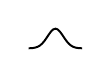
\begin{tikzpicture}[font=\small, >=stealth,yscale=0.25,xscale=0.2]
  \def\normaltwo{\x,{exp((-(\x)^2)/0.5)}}
  \draw[line width=0.25mm,domain=-1.7:1.7] plot (\normaltwo);
\end{tikzpicture}%
}

\newcommand{\ProductNode}{P}
\newcommand{\SumNode}{S}
\newcommand{\Leaf}{L}

\begin{document}
  

\tikzstyle{vertex}=[inner sep=0.01cm, circle, draw]
  \begin{tikzpicture} [scale=1, auto,>=latex]
    \path[use as bounding box] (-6.0,1.0) rectangle (6.3,-5);

    % Leaves
    \node[vertex, label=below:{$\Leaf_1$}](d1) at (-5.5, -4) {\usebox{\genericfilt}};
    \node[vertex, label=below:{$\Leaf_2$}](d2) at (-4.75, -4) {\usebox{\genericfilt}};
    \node[vertex, label=below:{$\Leaf_3$}](d3) at (-4.0, -4) {\usebox{\genericfilt}};
    \node[vertex, label=below:{$\Leaf_4$}](d4) at (-3.25, -4) {\usebox{\genericfilt}};
    \node[vertex, label=below:{$\Leaf_5$}](d5) at (-2.5, -4) {\usebox{\genericfilt}};
    \node[vertex, label=below:{$\Leaf_6$}](d6) at (-1.75, -4) {\usebox{\genericfilt}};
    \node[vertex, label=below:{$\Leaf_7$}](d7) at (-1.0, -4) {\usebox{\genericfilt}};
    \node[vertex, label=below:{$\Leaf_8$}](d8) at (-0.25, -4) {\usebox{\genericfilt}};
    \node[vertex, label=below:{$\Leaf_9$}](d9) at (0.5, -4) {\usebox{\genericfilt}};
    \node[vertex, label=below:{$\Leaf_{10}$}](d10) at (1.25, -4) {\usebox{\genericfilt}};
    \node[vertex, label=below:{$\Leaf_{11}$}](d11) at (2.0, -4) {\usebox{\genericfilt}};
    \node[vertex, label=below:{$\Leaf_{12}$}](d12) at (2.75, -4) {\usebox{\genericfilt}};
    \node[vertex, label=below:{$\Leaf_{13}$}](d13) at (3.5, -4) {\usebox{\genericfilt}};
    \node[vertex, label=below:{$\Leaf_{14}$}](d14) at (4.25, -4) {\usebox{\genericfilt}};
    \node[vertex, label=below:{$\Leaf_{15}$}](d15) at (5.0, -4) {\usebox{\genericfilt}};
    \node[vertex, label=below:{$\Leaf_{16}$}](d16) at (5.75, -4) {\usebox{\genericfilt}};

    % last layer
    \node[vertex, label=right:{$\ProductNode_3$}](j3) at (-5.125, -3) {\large$\bm\times$};
    \node[vertex, label=right:{$\ProductNode_4$}](j4) at (-3.615, -3) {\large$\bm\times$};
    \node[vertex, label=right:{$\ProductNode_5$}](j5) at (-2.105, -3) {\large$\bm\times$};
    \node[vertex, label=right:{$\ProductNode_6$}](j6) at (-0.625, -3) {\large$\bm\times$};
    \node[vertex, label=right:{$\ProductNode_7$}](j7) at (0.885, -3) {\large$\bm\times$};
    \node[vertex, label=right:{$\ProductNode_8$}](j8) at (2.395, -3) {\large$\bm\times$};
    \node[vertex, label=right:{$\ProductNode_9$}](j9) at (3.905, -3) {\large$\bm\times$};
    \node[vertex, label=right:{$\ProductNode_{10}$}](j10) at (5.415, -3) {\large$\bm\times$};

    % second last layer
    \node[vertex, label=right:{$\SumNode_2$}](s2) at (-4.25, -2) {\large$\bm+$};
    \node[vertex, label=right:{$\SumNode_3$}](s3) at (-1.25, -2) {\large$\bm+$};
    \node[vertex, label=right:{$\SumNode_4$}](s4) at (1.75, -2) {\large$\bm+$};
    \node[vertex, label=right:{$\SumNode_5$}](s5) at (4.75, -2) {\large$\bm+$};

    % second layer
    \node[vertex, label=right:{$\ProductNode_1$}](j1) at (-2.725, -1) {\large$\bm\times$};
    \node[vertex, label=right:{$\ProductNode_2$}](j2) at (3.25, -1) {\large$\bm\times$};

    % Root
    \node[vertex, label=right:{$\SumNode_1$}](s1) at (0, 0.5) {\large$\bm+$};

    % edges
    \draw [->] (s1) -- (j1);
    \draw [->] (s1) -- (j2);

    \draw [->] (j1) -- (s2);
    \draw [->] (j1) -- (s3);
    \draw [->] (j2) -- (s4);
    \draw [->] (j2) -- (s5);

    \draw [->] (s2) -- (j3);
    \draw [->] (s2) -- (j4);
    \draw [->] (s3) -- (j5);
    \draw [->] (s3) -- (j6);
    \draw [->] (s4) -- (j7);
    \draw [->] (s4) -- (j8);
    \draw [->] (s5) -- (j9);
    \draw [->] (s5) -- (j10);

    \draw [->] (j3) -- (d1);
    \draw [->] (j3) -- (d2);
    \draw [->] (j4) -- (d3);
    \draw [->] (j4) -- (d4);
    \draw [->] (j5) -- (d5);
    \draw [->] (j5) -- (d6);
    \draw [->] (j6) -- (d7);
    \draw [->] (j6) -- (d8);
    \draw [->] (j7) -- (d9);
    \draw [->] (j7) -- (d10);
    \draw [->] (j8) -- (d11);
    \draw [->] (j8) -- (d12);
    \draw [->] (j9) -- (d13);
    \draw [->] (j9) -- (d14);
    \draw [->] (j10) -- (d15);
    \draw [->] (j10) -- (d16);

 \end{tikzpicture}
\end{document}
